% Chapter Template

\chapter{Introduction}\label{Intro}   % Change X to a consecutive number; for referencing this chapter elsewhere, use \ref{Intro}

%----------------------------------------------------------------------------------------
%	SECTION 1
%----------------------------------------------------------------------------------------

\section{Epigenetics}

The genetic material is known to be modified during the life of an organism, possibly causing modifications in gene behavior. Far is known about mutations being a mayor player in genetic variation and the profiling of these variations has proved to be highly useful when studying diseases and evolutionary theory \cite{Wray2007}. In eukaryotes, there are in addition mechanisms in which the DNA can be modified without altering the molecular sequence, so called epigenetic mechanisms. As Conrad Waddington, who coined the term ``epigenetics'', defined: ``it is the branch of biology which studies the causal interactions between genes and their products, which bring the phenotype into being'' \cite{Waddington1942}. Such definition led to categorizing as epigenetics all biological phenomena which correlated the genetic material with the genetic products and were not explained entirely by the classic genetic studies. Further studies have revealed that epigenetic mechanisms can be modulated in response to external stimuli \cite{Liu2004,Backdahl2009}, entailing an overlay between DNA  and environment for the cells and organisms. Moreover, the epigenetic mechanisms behavior can vary for different stages of cell development \cite{Kiefer2007}, environmental changes \cite{Sutherland2003} or disease \cite{Jessberger2007}. In the same way genetic variability can be profiled, it is possible to decipher shared patterns for the epigenetic modifications in different scenarios and types of tissue.

\medskip

Due to the latest growth on research efforts and resources about the topic, we were able to characterized the inheritance of gene expression patterns not explained by the encoded information in the DNA sequence but through epigenetic modifications. High-throughput technologies such as Chromatin Inmunoprecipitation next-generation sequencing (ChIP-seq) or Whole-Genome Bisulfite sequencing (WGBS), allowed us to obtain an incredibly vast amount of information on epigenetic marks throughout the genome. It was then possible to determine the epigenome profile consisting of multiple chromatin states that activate or repress the gene expression in a local and cell-specific manner. This ``epigenomic profiling'' helped the understanding of cell differentiation, where even though the vast majority of cells in a multicellular organism share an identical genotype, the development of the various tissues generates stable but diverse profiles of gene expression, giving rise to the multiple cell types and differentiated cellular functions. In light of this, more specifically epigenetics may be defined as “the study of any potentially stable and, ideally, heritable change in gene expression or cellular phenotype that occurs without changes in Watson-Crick base-pairing of DNA” \cite{Goldberg2007}.

\medskip

The work on nucleic acids, chromatin and histone proteins led to the understanding of the DNA arrangement, as being wrapped around the histone proteins, and furthermore to the cytological distinction between euchromatin and heterochromatin \cite{Elgin1996}. It has been proved that post-translational modifications of the histones, such as methylation, acetylation or phosphorylation, can reshape the chromatin structural and functional properties instating the concept of turning ``on'' and ``off'' regions of the genetic material. A challenging yet feasible task is to characterize those configurations responsible for the repression, activation or modulation of the gene expression via epigenetic modifications, both in different tissues and also when affected by diseases as in the case of the cancer cells used in this study. For further understanding, it is essential to know about the diverse ways epigenetic mechanisms work and elucidate the correlation among them and to biological processes.

%-----------------------------------
%	SUBSECTION 1
%-----------------------------------
\subsection{Epigenetic modification types}

\subsubsection{Histone Modifications}

Chromatin is conformed by the DNA molecule and a range of binding proteins into which histones are included. The DNA molecule winds around an octamer of histones, formed by dimers of four core histones: H2A, H2B, H3 and H4. Histone N-terminal tails, specially long in Histone 3 (H3), are subject of chemical modifications, such as methylation or acetylation, modulating their spatial configuration and with it, the arrangement of the chromatin. First works on the subject, in particular on histone acetylation \cite{Schatz1964}, implied a close linkage between the histone modification state and the local gene activity. This assumption was afterwards supported by experiments on histone-tail mutations in \textit{Saccharomyces cerevisiae} \cite{Kayne1988}, hypoacetylation of the inactive X chromosome in female mammals \cite{Jeppesen1993}, as well as hyperacetylation of the twofold upregulated X chromosome in \textit{D. melanogaster} males \cite{Bone1994}. These major findings led to the compelling argument that histone modifications, along with DNA methylation, contribute to distinguish between euchromatin state and heterochromatin. Accordingly, depending on the particular histone modification profile, the chromatin can be arranged as euchromatin, which implies gene expression, or as heterochromatin, meaning the repression of the gene activity.

\medskip

Chromatin state at promoters is largely invariant across diverse cell types, whereas enhancers are marked with highly cell-type-specific histone modification patterns \cite{Heintzman2009}. As in methylation patterns, an aberrant histone modification pattern is associated with the development of cancer \cite{Barneda-Zahonero2012}. Histone deacetylases (HDACs) are implicated expecting both positive and negative effects on oncogenic and oncosuppressive mechanisms. Again, the importance of the histone modification patterns for the gene expression and the diseases associated with an aberrant histone modification profile, call our attention on the topic.

\subsubsection{DNA methylation}

DNA methylation is perhaps the best characterized chemical modification of chromatin and were detected as early as 1948 \cite{HOTCHKISS1948}. In mammals, nearly all DNA methylation occurs on cytosine residues of CpG dinucleotides. Regions of the genome that have a high density of CpGs are referred to as CpG islands, and DNA methylation of these islands correlates with transcriptional expression \cite{Deaton2011}. De novo or maintenance DNA methyltransferases (DNMTs) play a critical role in gene regulation, especially those associated with transposons and imprinted genes \cite{Goll2005}, by keeping the genomic patterns of cytosine methylation during embryogenesis and gametogenesis. Moreover, the formation of heterochromatin in several organisms is mediated partly by DNA methylation and its binding proteins together with RNA and histone modifications. DNA methylation takes part in many cellular processes including silencing of repetitive and centromeric sequences from fungi to mammals \cite{Partridge2002,Jones2012}; X chromosome inactivation in female mammals \cite{Weber2005}; and mammalian imprinting \cite{Bartolomei2011}, all of which can be stably maintained.

\medskip

As the other epigenetic mechanisms, DNA methylation is reversible and therefore DNA methylation patterns vary in time and space during differentiation \cite{Jones1980,Xie2013}. However, abnormal control of the methylation pattern was detected in cancer cells and may result in the generation of random modification patterns which may serve to unleash new genes for transcription \cite{Berdasco2010}. The abnormal methylation pattern can be either hypomehylated, which usually involves repeated DNA sequences, or hypermethylated which involves CpG islands \cite{Weber2005}. In the first case, oncogenes are activated whereas hypermethylation repress the transcription of the promoter regions of tumor suppressor genes, leading to gene silencing.

\subsubsection{RNA-Associated Silencing}

RNA silencing is another method to turn off genes when it is in form of antisense transcripts, noncoding RNAs or RNA interference. Antisense double-stranded RNA complementary to targeted mRNAs was detected as a method of Post-Transcriptional gene silencing (PTGS) for both cellular and viral genes in a sequence-specific manner \cite{Hamilton1999}. This kind of process is known as RNA-mediated interference or RNAi. Moreover, small non-coding RNAs were identified as potencial `templating' molecules for the location-specific epigenetic modifications. Several researches reported the involvement of small nuclear RNAs (snRNAs) in interacting with and presumably directing chromatin-modifying activities \cite{Mochizuki2002,Borges2015}. The snRNAs participate in a nuclear process known as `transcriptional gene silencing' (TGS) guiding the epigenetic machinery not only for heterochromatin assembly and gene silencing \cite{Grewal2003}, but also directing programmed DNA elimination \cite{Bernstein2005}.

\subsubsection{Alternative Splicing}

Alternative splicing is one major mechanism that makes the most of the precursor messenger RNAs (pre-mRNAs) by processing the pre-mRNA into a diverse array of mature mRNAs that encode distinct proteins. This phenomenon explains the high complexity of organisms as humans while they have a relatively small number of protein-coding genes. Alternative splicing of RNA leads to a variety of possible mRNA isoforms and proteins, which can have different, and often opposing, functions. Sequences called exons are regions of the pre-mRNA that are included in the mature mRNA, such as the protein-coding sequences and regulatory untranslated regions at either end of the mRNA.\@ Sequences called introns are the portions of the pre-mRNA that are removed during splicing. In alternative splicing, some sequences serve as exons under some conditions and are included in the final mRNA.\@ At other times, however, the alternative splicing process may exclude the same sequence, treating it as an intron and removing it from the mature mRNA.\@

\medskip

A critical finding regarding the prevalence of alternative splicing was that a majority of human genes produce a wide variety of messenger RNAs (mRNA) that in turn encode distinct proteins \cite{Johnson2003}. Scientists estimate that 15–60 percent of human genetic diseases involve splicing mutations, either through direct mutation of the splice-site signals or through disruption of other components of the splicing pathway \cite{Wang2007}. Therefore, understanding how the splicing machinery distinguish between exons, which are part of the mature mRNA, and introns, which are removed from the pre-mRNA, is of critical importance. Alternative splicing adds an extra layer of complexity, because regulatory sequences that sometimes designate an exon's inclusion into the mature mRNA dictate the exclusion of that exon under other conditions.

%-----------------------------------
%	SUBSECTION 2
%-----------------------------------

\subsection{Epigenomic modeling}

% Explain previous attempts on modeling the epigenetic profiles and where did they focus

% Origin of epigenetic modeling

Mentioned growth on epigenetics data availability, favored by the arise of NGS sequencing techniques, granted the possibility to create extensive descriptions on the different epigenetic marks for various samples. Moreover, the findings on the function of epigenetic modifications to modulate the chromatin arrangement provided a glimpse of the likeliness to characterize the relationships between chromatin states and gene expression profiles. Thanks to the contribution made to the two major public databases, the ENCODE (The ENCyclopedia of Dna Elements) \cite{Feingold2004} and the NIH Roadmap Epigenomics \cite{Bernstein2010}, this characterization becomes more accessible. Modeling the epigenetic modifications requires the development of computational tools which use the multiple types of data, such as DNA methylation, histone modification or Transcription Factors (TFs), in order to establish a correlation between the epigenomic assays and the biological activity. The main objectives of finding the specified models are both learn more about the biological association of epigenetic modifications and which predictions can be achieved from the models. The nature of the algorithms used to model epigenomics have been diverse but most of the proposed methods fall under unsupervised learning techniques of classification, which seek to devise patterns of chromatin modifications from the datasets alone, relying for it on multiple statistical techniques.

\medskip

A first proper mathematical attempt to model histone modification dynamics was made in \cite{Dodd2007}, where they characterized the bistable gene expression resulting from the alternative states of the chromosomal regions. They applied a simple stochastic model in which they divided the DNA into \~1.2 kb, corresponding to around 60 nucleosomes, and they consider either modified or unmodified nucleosomes from which they try to infer the state conversion of a region. Further contributions delved into the pattern-finding idea using more complete models such in ChromaSig \cite{Hon2008}. Nine different types of epigenetic marks were taken into account in order to find strong signals of correlation between the epigenetic signatures profile and the promoter and enhancer activity state. Nevertheless, the analysis worked on a pre-defined set of loci with high grade of epigenetic modifications from the ENCODE project pilot, representing only the 1\% of the human genome \cite{ENCODEProjectConsortium2007}. The essence of the method requires to calculate the likelihood for each loci towards being classified in a motif by using an euclidean distance measure. On account of the computational limitations, these methods could not be applied to study whole-genome marks and on multiple genomic assays.

\medskip

More recent tools are able to directly specify the combination of epigenetic modifications or `chromatin states' in a genome-wide fashion, making use of integrative models based on Hidden Markov Models (HMM) like in ChromHMM \cite{Ernst2010,Ernst2017} and EpicSeg \cite{Mammana2015}, or dynamic Bayesian networks like in Segway \cite{Hoffman2012}. ChromHMM software learns and characterizes the chromatin states from multiple ChIP-seq datasets by creating tracks of presence/absence vectors for the epigenetic mark in a k-binned genome. In such a way, genome-wide annotation is efficient but it misses the quantitative hand of the epigenetic mark reads, using only binary data. EpicSeg uses a similar angle in the analysis, however there is no need to pre-process the data as it uses raw read counts like observations in the analysis, which allows to define a valid discrete multivariate probability distribution and then solve the lost of quantitative data. For its part, Segway refuses the idea of genome segmentation and addresses the most probable sequence of chromatin states by means of a Dynamic Bayerian Network (DBN) at a 1-bp resolution. This approach can elucidate some limitations from previous methods such as missing data handling or finding the correct constrains for segments length.

\medskip

Yet, there are practical limitations essentially about the precondition to define the number of chromatin states beforehand, since this choice is arbitrary from the model and answers to biological interpretability of the results. Moreover, the algorithms mentioned above are computationally intensive and challenging to use without a sufficiently computational power. A relatively new statistical method called Non-Negative Matrix Factorization (NMF) \cite{Lee1999} has been applied to the problem in question of finding chromatin states from the reads of epigenetic modification marks \cite{Cieslik2014,Gandolfi2017}. NMF undertake the dimensionality problem on the genome-wide analysis of epigenetic tracks by approximating the dataset values through a reduced number of meaningful components \cite{Devarajan2008}. The method makes it possible to integrate multiple epigenetic marks to the characterization of chromatin combinatory patterns, and also allows to find an optimal number of distinct patterns based on the data. In both studies \cite{Cieslik2014,Gandolfi2017}, they applied NMF to matrices consisting on multiple epigenetic marks as columns and non-overlapping segments of the genome as rows, being the value of the cell equal to the read counts.

\medskip

In the first case, the segments used as rows correspond to multiple regions of TSS-proximal gene bodies since they contain epigenetic traces of transcription initiation and elongation. In the second case, they use bins of 200-bp, similar to the case in ChromHMM, in an attempt to approximate a single nucleosome with each bin. In this master thesis, aspects from these papers were used, extending the analysis to multiple cancer cell lines.

%----------------------------------------------------------------------------------------
%	SECTION 2
%----------------------------------------------------------------------------------------

\section{Non-negative Matrix Factorization}

Non-negative matrix Factorization reveals as a method to learn parts or components from high-dimensional data. In contrast to other matrix factorization methods such as Principal Component Analysis (PCA) or Vector Quantization (VQ), NMF does not learn holistic but part-based representations. In addition, NMF is constrained to have positive values as only additive combinations are considered \cite{Lee1999}. Basically, NMF consists on an approximation of an \(m \times n\) \(V\) matrix by the matrix multiplication of \(W\) (\(m \times k\)) and \(H\) (\(k \times n\)).

\begin{equation}
    V \approx W \times H
\end{equation}

This shall be accomplished by iteratively updating the rows and columns of \(W\) and \(H\) respectively. The constriction of the data to be positive also circumscribe the use of the method, though it has been applied in astronomy \cite{Ren2017}, language processing \cite{Bertin2010} or image processing \cite{Yang2007} among others. Gene expression, epigenetic modifications or mutation data have also been subject of analysis using NMF, considering the non-negativity of the data.

\medskip

Dealing with high dimensionality data using NMF implies taking certain decisions, starting from the choice of NMF dimensionality (number of \(k\) signatures). An important measure used for this task is the reconstruction error, calculated by comparing the original data value with the result of the multiplication of the factorized matrices \(W\) and \(H\). Some of the studies compare the reconstruction error produced by each defined \(k\) using the real data vs the one produced when taking random data, as it is the case in this analysis \cite{Frigyesi2008}. When examining the Residual Sum of Squares (RSS) as a function of \(k\), the RSS decreases with increasing \(k\) within the original dataset, however, this can be less the case for the random dataset. Ideally, for a given interval of \(k\) values, there ought to be an optimal \(k\) for which the slopes of the real and random data intersect. That is to say, we intend to find the highest \(k\), reducing the reconstruction error and improving the accuracy of the model, before being within the noise. Other studies use the cophenetic correlation coefficient, where the similarity between results from several runs is compared for each \(k\). In other words, the stability of the classification is studied choosing the highest \(k\) before the robustness of the results drops \cite{Brunet2004}.

\subsection{NMF algorithms}\label{NMFalgs}

Within NMF method we find several ways of solving the factorization problem of form \(V \approx W H\). Again, the non-negativity constrain makes previous factorization approaches not applicable and then new algorithms needed to be developed. First approaches \cite{Lee2001} were based on minimizing either the euclidean distance between \(V\) and \(WH\) such that

\begin{equation}
    \vert \vert V - WH \vert \vert ^2 = \sum_{ij} (V_{ij} - (WH)_{ij})^2
\end{equation}

or minimizing the divergence between \(V\) and \(WH\),

\begin{equation}
    D(V \vert \vert WH) = \sum_{ij}\left(V_{ij} \log \frac{V_{ij}}{(WH)_{ij}} - V_{ij} + (WH)_{ij} \right)
\end{equation}

as in both cases, the measure is lower bounded by zero and minimizes when \(V = WH\). Once the cost function for the minimization was defined, multiplicative rules were proposed as the procedure to update \(W\) and \(H\). A compelling property of the approximation is that (1.1) can be reformulated in a column or row-wise manner:

\begin{itemize}
    \item Update columns in \(H\): \(v \approx Wh\) when \(v\) represents a column in \(V\), \[v = (V_{1n}, \ldots , V_{Mn}) \in \mathbb{R}^M\], and \(h\) a column in \(H\), \[h = (H_{1n}, \ldots , H_{Kn}) \in \mathbb{R}^K\]
    \item Update rows in \(W\): \(v \approx wH\) when \(v\) represents a row in \(V\), \[v = (V_{1m}, \ldots , V_{Nm}) \in \mathbb{R}^N\] and \(w\) a row in \(W\) \[w = (W_{1m}, \ldots , W_{Km}) \in \mathbb{R}^K\]
\end{itemize}

Therefore, it is possible to iteratively update rows in \(W\) and then columns in \(H\). The multiplicative updates for \(H\) and \(W\) in the euclidean distance minimization were described with the next form \cite{Lee2001}:

\begin{equation}
    H_{kj} \leftarrow H_{kj} \frac{(W^T V)_{kj}}{(W^{T}WH)_{kj}	}
\end{equation}

\begin{equation}
    W_{ik} \leftarrow W_{ik} \frac{(V H^T)_{ik}}{(WHH^T)_{ik}}
\end{equation}

and the multiplicative updates for the divergence, based on Kullback-Leibler divergence, and subsequently applied to retrieve meaningful patterns from cancer gene expression data \cite{Brunet2004}, were described as follows:

\begin{equation}
    H_{kj} \leftarrow H_{kj} \frac{\sum_l \frac{W_{lk} V_{ij}}{(WH)_{ij}}}{\sum_l W_{lk}}
\end{equation}

\begin{equation}
    W_{ik} \leftarrow W_{ik} \frac{\sum_l \left[ \frac{H_{kl} V_{ij}}{(WH)_{il}} \right]}{\sum_l W_{kl}}
\end{equation}

Proofs of these theorems and convergence rules are further explained in \cite{Lee2001}. After these principle algorithms, some approaches were developed based on them in order to get sparser results \cite{Pascual-Montano2006} or include an intercept into the NMF fit \cite{Badea2008}.

\subsection{NMF and gene expression}

NMF was promptly introduced in bioinformatics as a method of dimensionality reduction of large-scale gene expression data \cite{Kim2003}. Here, functional relationships are yield from the analysis of 300 genome-wide expression measurements of yeast and compared with previous expertise. The 5346 genes analyzed in 300 samples were summarized in 50 patterns from which 12 were annotated with MIPS \cite{Mewes2002} functional categories, based on the frequency which genes from each category appeared in each of the signatures or patterns. In a similar way, NMF has also been applied to categorize tumor subtypes using 4651 human genes in 108 cases \cite{Frigyesi2008}, showing that NMF signatures may correspond specific disease gene expression patterns.

\subsection{NMF and mutations}

Besides finding shared patterns between diseases and gene expression, it has been shown that it is possible to characterize specific mutations produced in varied types of cancer \cite{Ramakrishna2012}. A catalogue of complete genomes for 21 primary breast cancer samples was sequenced and compared to the normal DNA of those same individuals. From these, 183,916 somatically acquired mutations were called and classified into 96 possible trinucleotide variations, composing the \(V\) matrix of \(183916 \times 21\) cells. NMF was then applied on this dataset and from the results they identified contribution of each of the mutational signatures in each of the patients, which yield similar arrangement for similar cancer types.

\medskip

Although the number of identified signatures was five, further on this number got reduced to only four signatures \cite{Alexandrov2013}. In such a way, mutational processes operative in cancer genomes were modeled with great accuracy by a combination of this four mutational signatures. This allowed to make predictions based on the signatures and the data, as well as understand more deeply the biological processes involved on the different types of cancer.

\subsection{NMF and epigenetics}

\medskip

\begin{figure}[h!]
    \centering
    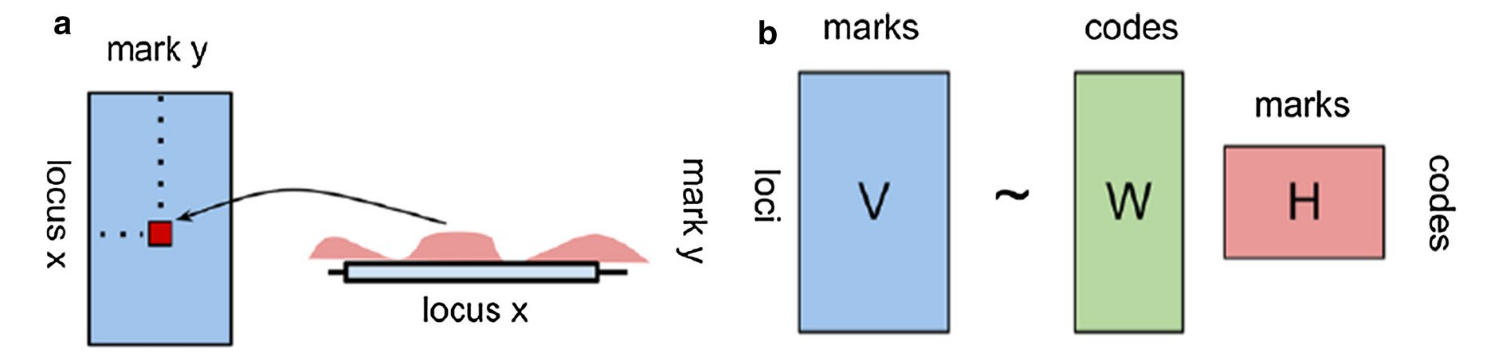
\includegraphics[width=\textwidth]{Figures/NMF/NMF_explanation.png}
    \caption[NMF of epigenetic data]{\textbf{NMF of epigenetic data}. Scheme of the NMF algorithm principle applied to epigenetic data. This is an image used recurrently in previous papers dealing with Non-Negative Matrix Factorization applied to biological data. \textbf{a:} The data values in the V matrix (blue), are obtained by calculating the normalized counts of each epigenetic mark (column) in every loci. We consider the 200-bp bins as loci in the present analysis. \textbf{b:} Represents the NMF algorithm principle, in which the V matrix described in \textbf{a} is factorized into two matrices; a W matrix containing the codes or signature weights for every bin, and an H matrix with signature weights for every epigenetic mark. As is is shown, we can recontruct the V matrix by multiplication of W and H}
    \label{fig:NMF_explanation}
\end{figure}

\medskip

The epigenetic modeling techniques explained before have shown the possibility to find genome-wide chromatin states based on the partition of the DNA. Nevertheless, they make the assumption that a small set of these chromatin states would be sufficient to describe the genomic expression, whereas several hundreds chromatin states have been estimated even with a small set of epigenetic marks used \cite{Ucar2011}. In addition, chromatin modifications tend to be highly correlated, hampering the task of assessing the importance of the chromatin marks and relating them to the biological mechanisms. NMF can be used in order to overcome these downsides by identifying combinatorial patterns of chromatin states.

\medskip

This application was initially presented as a way to get combinatorial patterns of epigenetic marks from integrated epigenetic data sets \cite{Cieslik2014}. They characterized a small amount of combinatorial patterns, which could be displayed and interpreted, were statistically capable of regression and classification tasks. Each row of the \(V\) matrix represents 2 kbp of regions flanking Transcription Start Sites (TSS) and columns represent the epigenetic marks used. In a case study for regression of \textit{Pol2} binding, ten epigenetic marks were used to identify seven quantitative epigenetic patterns. Using the 7 chromatin patterns in a regression model yield a performance of \( r^2 = 0.85 \), matching the one obtained by using 10 epigenetic marks but solving multicollinearity problems.

\medskip

Later on, functional classification of the epigenome was performed by adding more epigenetic marks and in this case, segmenting the DNA into 200 bp regions as an attempt to resemble one nucleosome with each 200-bp bin \cite{Gandolfi2017}. NMF was here applied to 13 different epigenetic marks over 833,738 significant bins in human embryonic stem cells, finding 7 epigenetic signals or chromatin profiles. These seven epigenetic signals were then labeled based on the related biological process and then used for a wide range of tasks: study the genomic distribution of the signatures, investigate their recovery power on genomic features, association with the gene expression \ldots



%----------------------------------------------------------------------------------------
%	SECTION 3
%----------------------------------------------------------------------------------------

\section{Objectives}

The main aim of this master thesis was to develop a computational pipeline capable of finding combinatorial patterns in the epigenomic data.

The absence of mapping information for the different epigenetic marks implied that a large proportion of the work consisted of processing the data. First, tools were developed for downloading epigenetic raw data and preparing the data for the analysis. The final employed data contained per-bin-counts for every epigenetic modification included in the analysis. Data from three cell types was used, hence three per-bin-counts matrices were produced.

\medskip

With the correct data, NMF algorithm was used on the assumption that we are able to find combinatorial patters or ``signatures''. The underlying idea of the present analysis is the ability of these signatures to summarize the epigenetic modifications states in two angles: (1) the interaction between the several epigenetic modification types, comprised by the \(H\) matrix, and (2) the interaction between the genomic regions, held by the \(W\) matrix. This been fulfilled, we can seek to relate the signatures with biological processes, as well as compare their differences among tissues.

\medskip

Over the present analysis, aspects from previous related analysis have been adopted, reproducing the arrangement of the data information for the processing step \cite{Gandolfi2017}, or segmenting the genome into 200-bp bins. Results show that there are similar chromatin signatures found for these tissues, suggesting a possible generalization of the chromatin profiles in normal and cancer cells. Moreover, some differences were found and are discussed in the upcoming sections.
